%%%%%%%%%%%%%%%%%%%%%%%%%%%%%%%%%%%%
% This is the template for submission to MICRO 2022
% The cls file is modified from 'sig-alternate.cls'
%%%%%%%%%%%%%%%%%%%%%%%%%%%%%%%%%%%%

\documentclass{sig-alternate}
\usepackage{mathptmx} % This is Times font
\usepackage{listings}
\usepackage{fancyhdr}
\usepackage{xcolor}
\usepackage[normalem]{ulem}
\usepackage[hyphens]{url}
\usepackage[sort,nocompress]{cite}
\usepackage[final]{microtype}
\usepackage[keeplastbox]{flushend}
\usepackage{subfig}
% Always include hyperref last
\usepackage[bookmarks=true,breaklinks=true,letterpaper=true,colorlinks,citecolor=blue,linkcolor=blue,urlcolor=blue]{hyperref}

\newcommand{\CommentOut}[1]{}
\newcommand\TODO[1]{\textcolor{red}{TODO #1}}

\definecolor{codegreen}{rgb}{0,0.6,0}
\definecolor{codegray}{rgb}{0.5,0.5,0.5}
\definecolor{codepurple}{rgb}{0.58,0,0.82}
\definecolor{backcolour}{rgb}{0.95,0.95,0.92}

\lstdefinestyle{mystyle}{
    backgroundcolor=\color{backcolour},   
    commentstyle=\color{codegreen},
    keywordstyle=\color{magenta},
    numberstyle=\tiny\color{codegray},
    stringstyle=\color{codepurple},
    basicstyle=\scriptsize,
    breakatwhitespace=false,         
    breaklines=true,                 
    captionpos=b,                    
    keepspaces=true,                 
    numbers=left,                    
    numbersep=5pt,                  
    showspaces=false,                
    showstringspaces=false,
    showtabs=false,                  
    tabsize=2
}

\lstset{style=mystyle}

% Ensure letter paper
\pdfpagewidth=8.5in
\pdfpageheight=11in

%%%%%%%%%%%---SETME-----%%%%%%%%%%%%%
\newcommand{\microsubmissionnumber}{XXX}
%%%%%%%%%%%%%%%%%%%%%%%%%%%%%%%%%%%%

\fancypagestyle{firstpage}{
  \fancyhf{}
  \renewcommand{\headrulewidth}{0pt}
  \fancyhead[C]{\vspace{10pt}\normalsize{MICRO 2022 Submission
      \textbf{\#\microsubmissionnumber} -- Confidential Draft -- Do NOT Distribute!!}\\\vspace{-25pt}} 
  \fancyfoot[C]{\thepage}
}

\pagenumbering{arabic}

%%%%%%%%%%%---SETME-----%%%%%%%%%%%%%
\title{Treebeard : A Compiler for Decision Forest Inference} 
%%%%%%%%%%%%%%%%%%%%%%%%%%%%%%%%%%%%

\begin{document}
\maketitle
\thispagestyle{firstpage}
\pagestyle{plain}



%%%%%% -- PAPER CONTENT STARTS-- %%%%%%%%
\begin{abstract}
  Decision tree ensembles are commonly used machine learning models
  generated by machine learning techniques like gradient boosting and random forests. 
  These models are used in a wide range of applications and are deployed at scale
  (run repeatedly on billions of data items). Several libraries such as XGBoost, 
  LightGBM, and Sklearn expose algorithms for both training and inference with 
  decision tree ensembles. While these libraries 
  incorporate a limited set of hardware-specific optimizations,
  they do not specialize the inference code to the model being used, 
  leaving significant performance on the table.

  This paper presents a compiler-based approach that automatically generates  
  efficient code for decision tree inference. 
  It develops Treebeard, an extensible compiler, which progressively lowers  
  inference code to LLVM IR through multiple intermediate abstractions.
  By applying model-specific optimizations at the higher levels, loop
  optimizations at the middle level, and machine-specific optimizations lower down,
  Treebeard can specialize inference code for each model on each supported
  hardware target. To improve model inference performance, Treebeard performs several 
  novel optimizations such as tree tiling, tree walk unrolling, and tree walk interleaving.
 
  We implement Treebeard using the MLIR compiler infrastructure and
  demonstrate the utility of Treebeard by evaluating it on a diverse set of
  tree ensemble models. Experimental evaluation demonstrates that Treebeard optimizations 
  improve average latency over a batch of inputs by 2.2X over our baseline version. 
  Further, Treebeard is significantly faster than %% other frameworks like
  XGBoost and Treelite in both single-core (2.8X and 5.1X respectively) and multi-core
  (3.2X and 2.6X respectively) settings.
\end{abstract}

\section{Introduction}
% Decision trees are among the most widely used ML models. Cite Kaggle and looking glass 
Decision tree ensembles are one of the most popular classes of machine learning models \cite{KaggleSurvey,LookingGlass}.
They are generated by machine learning techniques like gradient boosting and random forests. 
The Kaggle state of data science and machine learning survey \cite{KaggleSurvey} shows that 
these are the most widely used classes of models among data scientists. An analysis of 
several machine learning pipelines that are in production use in a real large scale web company showed that 
gradient boosting machines and random forests were the two most widely used ML algorithms in the company \cite{LookingGlass}.
Not only are decision tree based models widely used, they are also used in a diverse range of 
applications\cite{DecisionTreesOverview}. GBM models were used in the CERN large hadron collider
to classify particles based on the data collected from the collider\cite{LHCModel}. Other applications 
include search engines\cite{YahooSearch}, prediction of the financial performance of companies\cite{Finance},
medical diagnostics\cite{Med1, Med2} and recommendation and notification systems\cite{Facebook}.

% Decision tree ensemble overview
To compute the prediction of a decision tree on an input row $x$\footnote{An input row is a
vector of numbers.}, a path from the root to leaf is computed.
Each node of a decision tree has a threshold value $v$ and a feature index (or column index) $i$.
At a node, if $x_i < v$, then 
the walk moves to the left child. If not, we move to the right child. When a leaf is reached, 
the value of the leaf is returned as the prediction of the tree. 
Most decision tree based techniques combine several trees into a forest (or ensemble) to improve prediction accuracy.
To compute the prediction of the forest, the prediction of each tree is computed and these predictions are 
then combined (usually by adding them). 

% Inference on decision trees is hard 
% Pointer chasing -- cache performance, branch prediction, dependency stalls, not easy to vectorize
Given the wide spread use of decision tree ensembles, the ability to perform high throughput and low latency inference is important.
\TODO{AP Since we don't talk about latency or throughput explicitly, should we be saying this?}
However, optimizing the tree walks required for decision tree inference on modern CPUs is not straight-forward. 
Firstly, naively implemented tree walks have poor spatial and temporal locality and therefore poor cache performance \cite{FAST,MilindTreeVectorization}.
Additionally, since the decision of which node to evaluate next can only be made after evaluating the current node,
true dependencies between instructions cause several pipeline stalls. Also, using SIMD instructions to accelerate 
tree walks is extremely challenging \cite{MilindTreeVectorization}.

Several systems like XGBoost\cite{XGBoost}, LightGBM\cite{LightGBM} and Sklearn\cite{Sklearn} implement
decision tree ensemble inference. These are libraries and implement some optimizations. However, these optimizations are hand
coded and need to be manually rewritten or redesigned for every target that is supported. Also, these 
systems cannot apply specialize inference code depending on the model. A compiler based approach is 
needed to address these problems. However, existing compilers only support fixed code generation techniques\cite{Treelite, Hummingbird}.
To fill the need for an extensible compiler infrastructure for decision forest ensembles, we design and 
build \Treebeard{}\footnote{In J. R. R. Tolkein's The Lord of the Rings, Treebeard was the oldest of the Ents left in Middle-earth, an 
ancient tree-like being who was a ``shepherd of trees''.}, an optimizing compiler for decision tree ensemble inference.
Our motivations for building \Treebeard{} are as follows. 
\begin{enumerate}
  \item Existing libraries \cite{XGBoost, Treelite, LightGBM, VPred} perform specific optimizations and are hard to maintain as hardware evolves. 
  Additionally, they cannot tailor inference code to the specific model being used. Past work has identified that the optimizations required change with the model
  and architectural parameters like cache size\cite{CacheConscious1, CacheConscious2, VPred}. 
  \item The repeated effort to optimize and maintain libraries on several targets is prohibitive. The proliferation of new architectures
  further exacerbates this problem. Compilers have been successful in alleviating this problem in other domains\cite{Halide, TVM}.
  However, no such compiler infrastructure currently exists for decision tree ensembles.
  \item Currently, no system exists that allows a thorough exploration of the optimization space for decision tree ensemble inference. 
  Compilers have been successful in addressing this problem with ML models like DNNs \cite{TVM, Tiramisu, XLA}. However, compiler techniques for
  decision tree ensembles are less well studied.
\end{enumerate}

We make the following contributions.
\begin{enumerate}
  \item We design and build \Treebeard{}, an extensible compiler infrastructure for decision tree model inference. The 
  infrastructure is built to allow exploration of optimization and code generation techniques. \TODO{Is this claim too grand?}
  \item We develop a general infrastructure for the vectorization of decision tree walks based on grouping tree nodes into ``tiles''.
   This includes general support for code generation and the in-memory representation of tiled trees. The infrastructure can be 
   used to tile trees based on different cost functions.
  \item We show that trees can be tiled using different cost functions. We present two novel tiling methods that are implemented
  using the general tiling infrastructure. 
  \item We design and implement various model and loop transformations that significantly improve generated inference code performance 
  to show the power of the proposed framework.
\end{enumerate}



\section{Treebeard Overview}
Figure \ref{Fig:CompilerStructure} shows the high level structure of \Treebeard{}. 
The input to \Treebeard{} is a serialized decision tree ensemble. 
%% Popular frameworks like XGBoost and LightGBM are supported and the system is easily extensible to other frameworks.
Given an input model our compiler generates optimized inference code. Specifically it generates a 
callable batch inference function \texttt{predictForest} that, given an array of input rows, computes an
array of model predictions. 
 
\Treebeard{} specializes the code generated for inference by progressively optimizing and lowering a 
high level representation of the \texttt{predictForest} function down to LLVM IR \cite{LLVM}.
%% By \textbf{\emph{lowering}}, we mean 
\textbf{\emph{Lowering}} is the process of transforming an operation at a higher 
abstraction to a sequence of operations at a lower abstraction. Optimizations in \Treebeard{} 
are implemented using a combination of annotation and lowering. An operation at a higher 
abstraction is annotated with attributes that indicate what kind of optimization is 
to be performed while lowering it. The lowering transformation uses this information to generate 
optimized lower level code. For example, tree tiling and loop ordering (figure \ref{Fig:Overview} 
shows two possible loop orders -- one tree at a time and one row at a time) are decided 
at the highest abstraction. These decisions are communicated to the lowering pass 
which explicitly encodes them in the lowered IR as shown in Figure \ref{Fig:Overview}.

%Treebeard first constructs a high level representation of the decision forest inference operation.
\Treebeard{}'s IR has three abstraction levels as shown in Figure \ref{Fig:Overview}.  
At the highest level (HIR), the input model is represented as a collection of binary trees. This is shown 
in the second row of Figure \ref{Fig:Overview}. At this level of abstraction,
\Treebeard{} tiles nodes together to transform a binary tree into an $n$-ary tree 
and decides what order trees are to be traversed in. In the example in the figure, 
trees are tiled with a tile size of 2. Tiling is indicated using colored elipses drawn 
around nodes that are in the same tile. Tree reordering is another transformation that is performed at this abstraction. 
One objective of tree reordering is to group identically structured trees so that they can share the same traversal code
to improve locality in the instruction cache.  Alternative objectives for reordering can easily be supported.
With the tiling shown in Figure \ref{Fig:Overview}, Tree1 and Tree3 have depth 1, while Tree2 has a depth of 2.
Therefore, the trees are reordered so that Tree1 and Tree3 are together. 

The high level IR is then lowered to a mid-level IR (MIR). The aim of MIR is 
to allow optimizations that are independent of the final memory layout of the model. 
The lowering to MIR performs loop transformations like loop tiling, permutation, parallelization and unrolling.
At this level of the IR (the third row in Figure \ref{Fig:Overview}),
the order in which trees, input row pairs are walked is explicitly represented in the IR using loop nests.
Figure \ref{Fig:Overview} shows two possible ways that loop nests could be generated -- the first
walks all rows for one tree before moving to the next tree while the second walks all trees for 
one row before moving to the next row. Another aspect handled by this lowering is the fissing of 
loops to make sure that trees with the same structure share code. Here, both versions of MIR shown 
ensure that Tree1 and Tree3 share the same traversal code, while traversal code for Tree2 is different.
Additionally, tree walk optimizations, such as tree walk unrolling (shown in figure \ref{Fig:Overview}) and 
peeling are performed on the MIR.

\Treebeard{} then further lowers the IR to explicitly represent the memory layout of the model. Buffers to hold model 
values are inserted into the generated code and all tree operations in the mid-level IR are lowered to explicitly 
reference these buffers. Additionally, at this level of the IR, \Treebeard{} generates vectorized code to take 
advantage of SIMD instructions where applicable. Finally, the inference function is translated to LLVM IR and 
JIT compiled to executable code. 

%The following sections describe each level of the IR and their lowering in more detail.

\begin{figure}
  \centering
  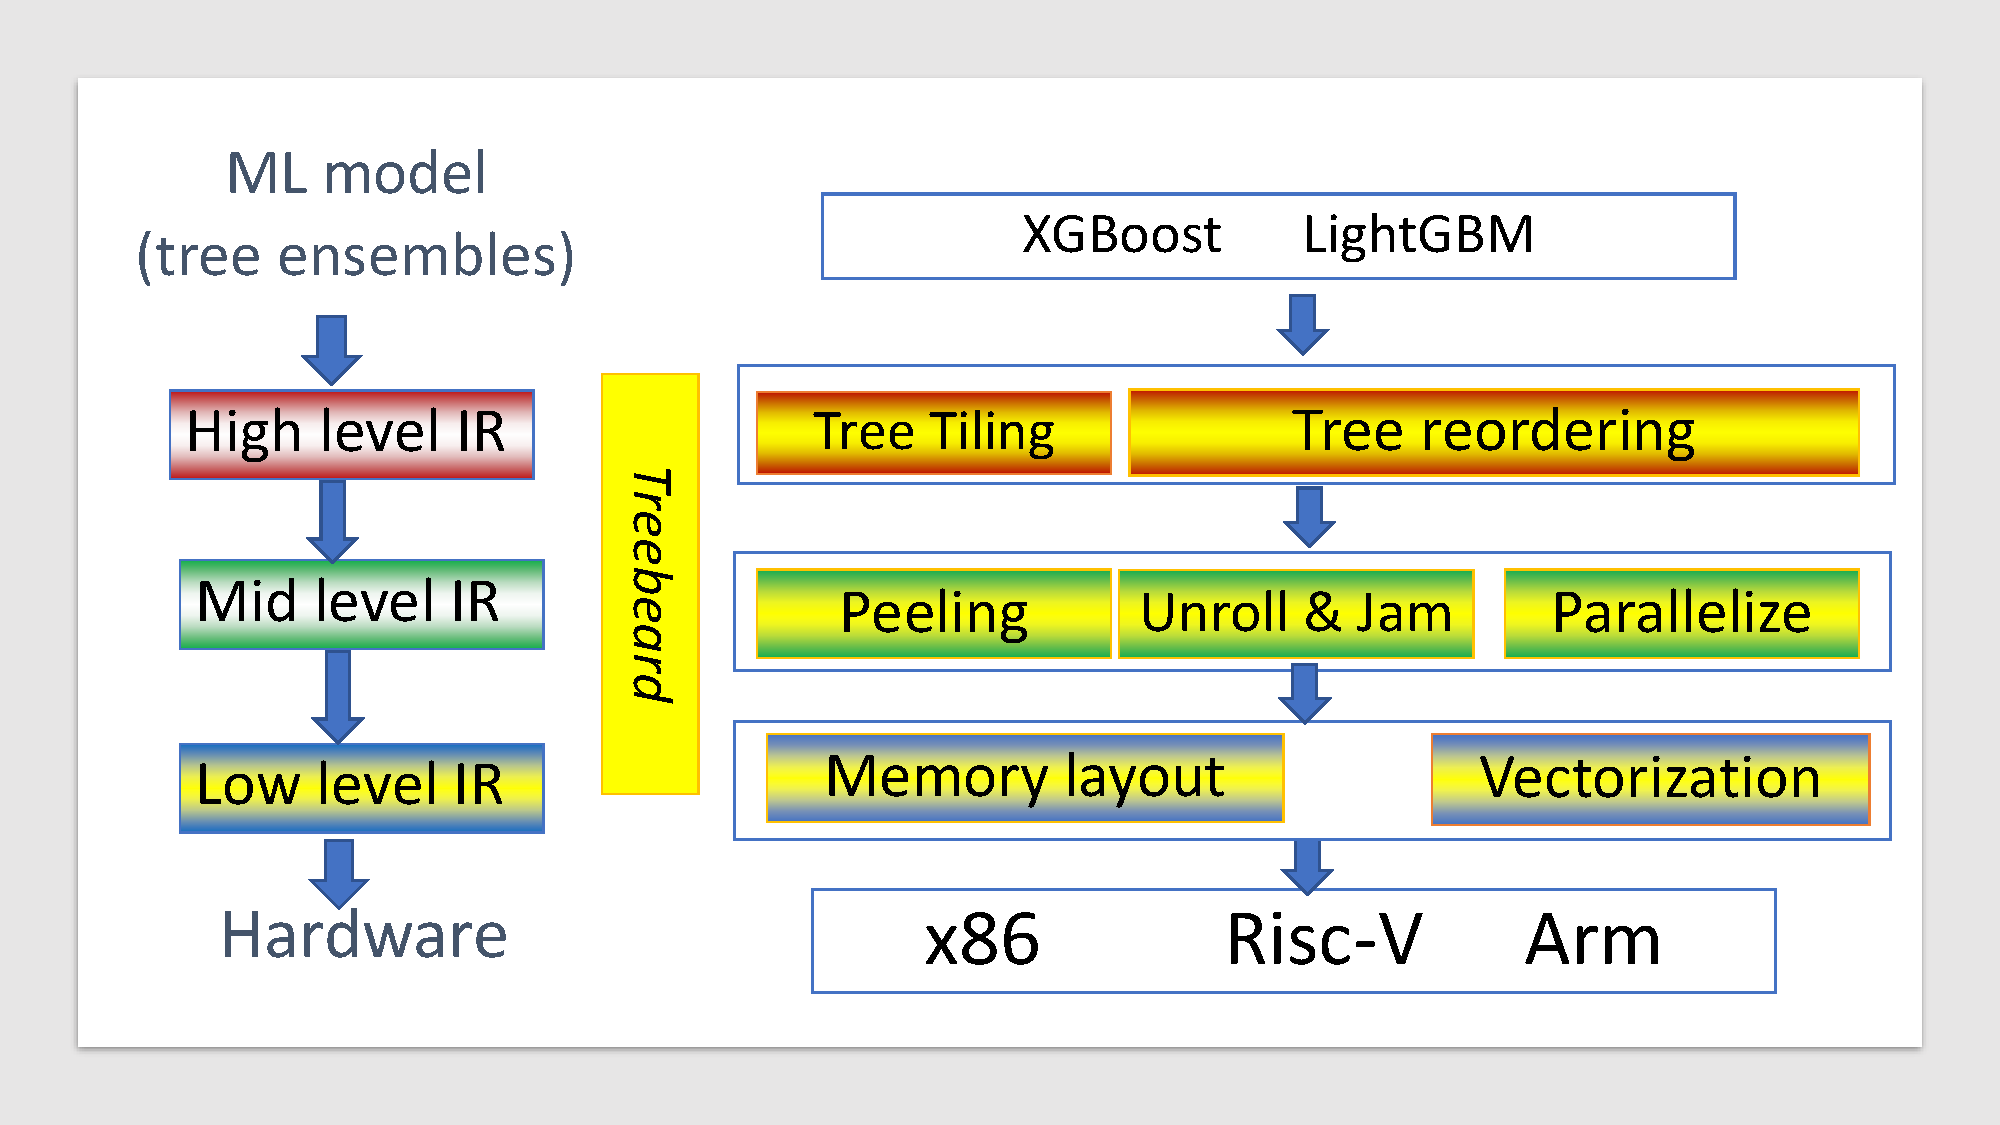
\includegraphics[width=\linewidth]{figures/compiler.pdf}
  \caption{Treebeard compiler structure}
  \label{Fig:CompilerStructure}
\end{figure}

\begin{figure*}
  \centering
  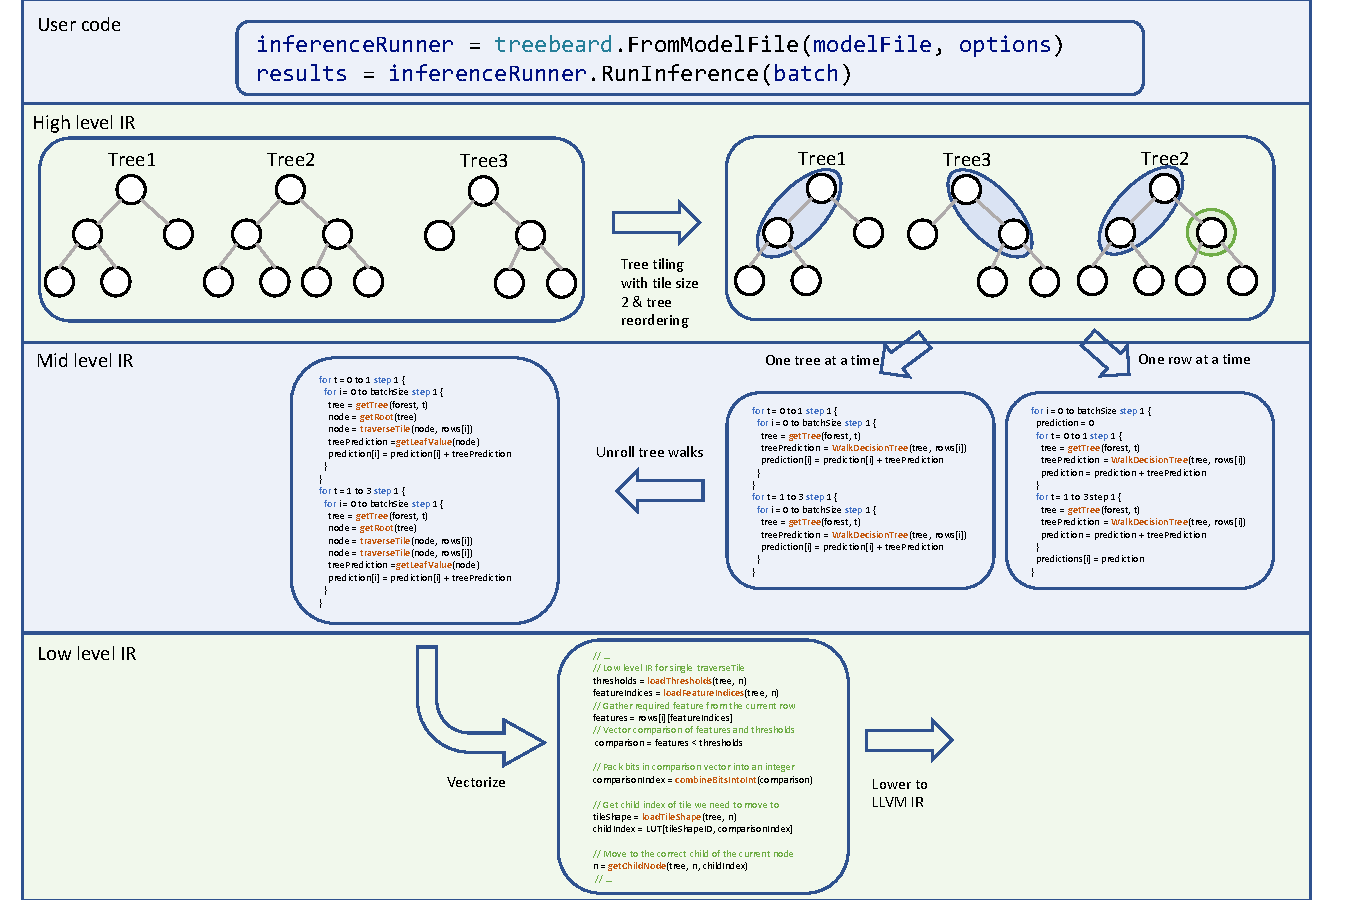
\includegraphics[width=\textwidth]{figures/OverviewExample.pdf}
  \caption{\Treebeard{} IR lowering and optimization details. The three abstraction levels in Treebeard's IR are shown. The
           high level IR is a tree based IR to perform model level optimization, the mid-level IR is for
           loop optimizations that are independent of memory layout and the low level IR allows us to perform
           vectorization and other memory layout dependent optimizations.}
  \label{Fig:Overview}
\end{figure*}



%\TODO{Should we describe the dialect's type system?}
% \TODO{Kr : consider focusing on the example instead of verbose description of optimizations. This section can be short, descriptions can come in later sections.}
% \subsection{High Level IR}
% As a first step Treebeard parses the input and generates a single MLIR operation, \texttt{predictForest} that represents inference using the input model on a set of rows. 
% At this level the operator simply contains a collection of binary trees. Two optimizations, tiling and tree ordering are applied at this level. The objective of tiling is to group nodes together so that the tree can be walked one tile at a time instead of one node at a time. We demonstrate that tiling can specialize the traversal of individual trees to either balance heavily skewed trees or proritize walks leading to higher probability leafs. Figure~\ref{ttile} shows examples of the tiling transformation. \TODO{kr: draw and explain example}. The objective of tree reordering is to group identically structured trees so that they can share the same traversal code. The predictForest function is now lowered to MIR with separate loop nests generated for traversing groups of identical trees. The generated MIR code is as shown below. 
% \TODO{show unoptimized loop nest as a listing}.

%The operation contains within it a tree based representation of the model that can be manipulated by optimizing transformations. Transformations on the model such as tiling, tree reordering and leaf padding are done at this level. The structure of the loop nest to walk the iteration space of trees and inputs is also decided at this level of the IR. \TODO{Should we mention that there is a scheduling language to decide this?}
% \begin{lstlisting}[language=C++]
% func Predict(float rows[batchSize]) {
%   predictions = predictForest(rows) 
%   return rows
% }
% \end{lstlisting}

% \subsection{Mid Level IR}
% The Mid Level IR optimizes the loop structures and tree walks. Firstly, the order in which the iteration space of trees and inputs is walked is determined and by re-ordering the loop nesting if necessary. Also, operations such as \texttt{isLeaf}, \texttt{traverseTile}, \texttt{getLeafValue} are introduced so that the traversal of trees explicitly represented. The following listing shows the IR for inference using a model with four trees on an input batch with two rows. The listed IR walks all trees for one input row before moving to the next row. One important point to note here is that details such as the data structure used for the trees are not explicitly encoded in the IR. This allows us to reuse optimization and lowering passes on this level of the IR regardless of what the final in memory representation of the model is.

% \begin{lstlisting}[style=c++]
%   // Constant that represents the model being compiled
%   forest = ensemble(...)
%   for i = 0 to 2 step 1 {
%     prediction = 0
%     for t = 0 to 4 step 1 {
%       tree = getTree(forest, t) 
%       node = getRoot(tree)
%       while (isLeaf(tree, n)==false)  do {
%         node = traverseTreeTile(tree, node, rows[i])
%       }
%       treePrediction = getLeafValue(tree, node)
%       prediction = prediction + treePrediction
%     }
%     predictions[i] = prediction
%   }
% \end{lstlisting}

% The IR listed above is a simplification of the actual IR. The actual IR is strongly typed and in SSA form.

% \subsection{Low Level IR}
% The IR is finally lowered to a form where the in memory representation of the model is made explicit. Buffers to hold the model values are inserted into the generated code and all tree operations in the mid-level IR are lowered to explicitly reference these buffers. The semantics of all operations are made explicit. For example, \texttt{traverseTreeTile} is lowered into a series of operations to load thresholds, feature indices and features, compare the features with the thresholds and compute the next node to evaluate. This IR is then lowered directly to LLVM IR and JITted.





\CommentOut{
\begin{abstract}

  This document is intended to serve as a sample for submissions to the 55\textsuperscript{th} IEEE/ACM International Symposium on Microarchitecture\textsuperscript{\textregistered} (MICRO 2022). We provide some guidelines that authors should follow when submitting papers to the conference.  This format is derived from the ACM sig-alternate.cls file, and is used with an objective of keeping the submission version similar to the camera-ready version.

\end{abstract}

\section{Introduction}

This document provides instructions for submitting papers to the 55\textsuperscript{th} IEEE/ACM International Symposium on Microarchitecture\textsuperscript{\textregistered} (MICRO 2022).  In an effort to respect the efforts of reviewers and in the interest of fairness to all prospective authors, we request that all submissions to MICRO 2022 follow the formatting and submission rules detailed below. Submissions that violate these instructions may not be reviewed, at the discretion of the program chairs, in order to maintain a review process that is fair to all potential authors. 

This document is itself formatted using the MICRO 2022 submission format. The content of this document mirrors that of the submission instructions that appear on the conference website. All questions regarding paper formatting and submission should be directed to the program chairs.

\subsection{Format Highlights}
\begin{itemize}
\item Paper must be submitted in printable PDF format.
\item Text must be in a minimum 10pt font, see Table~\ref{table:formatting}.
\item Papers must be at most 11 pages, not including references.
\item No page limit for references.
\item Each reference must specify {\em all} authors (no {\em et al.}).
\item Author anonymity must be fully preserved, including in any referenced artifacts (e.g., GitHub repository).
\end{itemize}

\subsection{Paper Evaluation Objectives} 
The committee will make every effort to judge each submitted paper on its own merits. There will be no target acceptance rate. We expect to accept a wide range of papers with appropriate expectations for evaluation---while papers that build on significant past work with strong evaluations are valuable, papers that open new areas with less rigorous evaluation are equally welcome and especially encouraged.

\section{Paper Preparation Instructions}

\subsection{Paper Formatting}

Papers must be submitted in printable PDF format and should contain a {\em maximum of 11 pages} of single-spaced two-column text, {\bf not including references}.  You may include any number of pages for references, but see below for more instructions.  If you are using \LaTeX~\cite{lamport94} to typeset your paper, then we suggest that you use the template here: \href{https://www.microarch.org/micro55/submit/micro55-latex-template.zip}{\LaTeX~Template}. This document was prepared with that template. Note that the template and sample paper may render slightly differently on different \LaTeX~engines, due to typesetting changes between versions. If you use a different software package to typeset your paper, then please adhere to the guidelines given in Table~\ref{table:formatting}. 

\begin{scriptsize}
\begin{table}[h!]
  \centering
  \begin{tabular}{|l|l|}
    \hline
    \textbf{Field} & \textbf{Value}\\
    \hline
    \hline
    File format & PDF \\
    \hline
    Page limit & 11 pages, {\bf not including}\\
               & {\bf references}\\
    \hline
    Paper size & US Letter 8.5in $\times$ 11in\\
    \hline
    Top margin & 1in\\
    \hline
    Bottom margin & 1in\\
    \hline
    Left margin & 0.75in\\
    \hline
    Right margin & 0.75in\\
    \hline
    Body & 2-column, single-spaced\\
    \hline
    Space between columns & 0.25in\\
    \hline
    Line spacing (leading) & 11pt \\
    \hline
    Body font & 10pt, Times\\
    \hline
    Abstract font & 10pt, Times\\
    \hline
    Section heading font & 12pt, bold\\
    \hline
    Subsection heading font & 10pt, bold\\
    \hline
    Caption font & 9pt (minimum), bold\\
    \hline
    References & 8pt, no page limit, list \\
               & all authors' names\\
    \hline
  \end{tabular}
  \caption{Formatting guidelines for submission.}
  \label{table:formatting}
\end{table}
\end{scriptsize}

{\em Please ensure that you include page numbers with your submission}. This makes it easier for the reviewers to refer to different parts of your paper when they provide comments. Please ensure that your submission has a banner at the top of the title page, similar to this document, which contains the submission number and the notice of confidentiality.  If using the template, just replace XXX with your submission number.

\subsection{Content}

Reviewing will be {\em double blind} (no author list); therefore, please do not include any author names on any submitted documents except in the space provided on the submission form.  You must also ensure that the metadata included in the PDF does not give away the authors. You must fully anonymize any links to artifacts (e.g., GitHub repository) and remove any links to artifacts that cannot be fully anonymized. {\bf Papers that violate the anonymization policy may be rejected without review} at the discretion of the program chairs.


If you are improving upon your prior work, refer to your prior work in the third person and include a full citation for the work in the bibliography.  For example, if you are building on {\em your own} prior work in the papers \cite{nicepaper1,nicepaper2,nicepaper3}, you would say something like: "While the authors of \cite{nicepaper1,nicepaper2,nicepaper3} did X, Y, and Z, this paper additionally does W, and is therefore much better."  Do NOT omit or anonymize references for blind review.  There is one exception to this for your own prior work that appeared in IEEE CAL, arXiv, workshops without archived proceedings, etc.\, as discussed later in this document.

\noindent\textbf{Figures and Tables:} Ensure that the figures and tables are legible.  Please also ensure that you refer to your figures in the main text.  Many reviewers print the papers in gray-scale. Therefore, if you use colors for your figures, ensure that the different colors are highly distinguishable in gray-scale.

\noindent\textbf{References:}  There is no length limit for references. {\em Each reference must explicitly list all authors of the paper.  Papers not meeting this requirement will be rejected.} Authors of NSF proposals should be familiar with this requirement. Knowing all authors of related work will help find the best reviewers. Since there is no length limit for the number of pages used for references, there is no need to save space here.

\section{Paper Submission Instructions}

\subsection{Guidelines for Determining Authorship}
IEEE guidelines dictate that authorship should be based on a {\em substantial intellectual contribution}. It is assumed that all authors have had a significant role in the creation of an article that bears their names. In particular, the authorship credit must be reserved only for individuals who have met each of the following conditions:

\begin{enumerate}
\item Made a significant intellectual contribution to the theoretical development, system or experimental design, prototype development, and/or the analysis and interpretation of data associated with the work contained in the article;

\item Contributed to drafting the article or reviewing and/or revising it for intellectual content; and

\item Approved the final version of the article as accepted for publication, including references.
\end{enumerate}

A detailed description of the IEEE authorship guidelines and responsibilities is available \href{https://www.ieee.org/publications_standards/publications/rights/Section821.html}{here}. Per these guidelines, it is not acceptable to award {\em honorary } authorship or {\em gift} authorship. Please keep these guidelines in mind while determining the author list of your paper.

\subsection{Declaring Authors}
Declare all the authors of the paper upfront. Addition/removal of authors once the paper is accepted will have to be approved by the program chairs, since it potentially undermines the goal of eliminating conflicts for reviewer assignment.

\subsection{Areas and Topics}
Authors should indicate these areas on the submission form as well as specific topics covered by the paper for optimal reviewer match. If you are unsure whether your paper falls within the scope of MICRO, please check with the program chairs -- MICRO is a broad, multidisciplinary conference and encourages new topics.

\subsection{Revision of Previously-Reviewed\\ Manuscript}
If the manuscript has been previously reviewed and rejected and is now being submitted to MICRO, the authors have an option of providing a letter explaining how the paper has been revised for this current submission. We expect this revision information to improve both the submission and the review process. Authors choosing to provide such a letter have control over who has access to it by specifying one of the following options:

\begin{enumerate}
\item Shared with all reviewers of the paper 
\item Shared with reviewers who declare that they reviewed a prior version and who request the revision information
\item Not shared with any PC member but available to the program chairs
\end{enumerate}

We encourage you to keep this letter concise and optionally append additional information, such as a version of the paper that highlights the differences or any other material of your choice.

\subsection{Declaring Conflicts of Interest}
Authors must register all their conflicts for their paper submission. Conflicts are needed to ensure appropriate assignment of reviewers. {\bf If a paper is found to have an undeclared conflict that causes a problem OR if a paper is found to declare false conflicts in order to abuse or ``game'' the review system, the paper may be rejected without review.} We use the following conflict of interest guidelines for determining the conflict period for MICRO 2022.  Please declare a conflict of interest (COI) with the following people for any author of your paper:

\begin{enumerate}
\item Your Ph.D. advisor(s), post-doctoral advisor(s), Ph.D. students,
      and post-doctoral advisees, forever.
\item Family relations by blood or marriage, or their equivalent,
      forever (if they might be potential reviewers).
\item People with whom you have collaborated in the last FOUR years, including:
  \begin{itemize}
  \item co-authors of accepted/rejected/pending papers
  \item co-PIs on accepted/rejected/pending grant proposals
  \end{itemize}
\item Ongoing collaboration that has not yet resulted in a paper or proposal submission. Justification may be queried.
\item When there is a direct funding relationship between an author and the potential reviewer (e.g., the reviewer is a sponsor of an author's research on behalf of his/her company or vice versa) in the last FOUR years.
\item People (including students) who shared your primary institution(s) in the last FOUR years.
\item Other relationships, such as close personal friendship, that you think might tend
to affect your judgment or be seen as doing so by a reasonable person familiar
with the relationship.
\end{enumerate}

We would also like to emphasize that the following scenarios do {\em not} constitute a conflict:
\begin{enumerate}
\item Authors of previously-published, closely related work on that basis alone.
\item ``Service'' collaborations such as co-authoring a report for a professional organization, serving on a program committee, or co-presenting tutorials.
\item Co-authoring a paper that is a compendium of various projects with no true collaboration among the projects.
\item People who work on topics similar to or related to those in your papers.
\item Collaborators on large funded projects where there is no close collaboration and no joint benefit in the paper being accepted.
\end{enumerate}

We hope to draw most reviewers from the program committee, but others
from the community may also write reviews. {\bf Please declare all your conflicts (not just restricted to the PC).} When in doubt, please contact the program chairs.

%Please note that all paper submissions require all authors to electronically sign a statement confirming their best effort to accurately identify potential reviewers with a conflict of interest, and importantly also {\bf assuring that each author will make no explicit attempt to directly or indirectly influence any reviewer opinion or decision about the submitted paper}. Importantly, we do not consider technical discussion of a paper's content or any other sharing of content from the paper to violate the above policy. 


\subsection{Concurrent Submissions and Workshops}

By submitting a manuscript to MICRO 2022, the authors guarantee that the manuscript has not been previously published or accepted for publication in a substantially similar form in any conference, journal, or the archived proceedings of a workshop (e.g., in the ACM/IEEE digital library) -- see exceptions below. The authors also guarantee that no paper that contains significant overlap with the contributions of the submitted paper will be under review for any other conference or journal or an archived proceedings of a workshop during the MICRO 2022 review period. Violation of any of these conditions will lead to rejection.

The only exceptions to the above rules are for the authors' own papers in (1) workshops without archived proceedings such as in the ACM/IEEE digital library (or where the authors chose not to have their paper appear in the archived proceedings), or (2) venues such as IEEE CAL or arXiv where there is an explicit policy that such publication does not preclude longer conference submissions.  In all such cases, the submitted manuscript may ignore the above work to preserve author anonymity. This information must, however, be provided on the submission form -- the program chairs will make this information available to reviewers if it becomes necessary to ensure a fair review.  As always, if you are in doubt, it is best to contact the program chairs.


Finally, the ACM/IEEE Plagiarism Policy (\href{http://www.acm.org/publications/policies/plagiarism_policy}{here} and \href{https://www.ieee.org/publications_standards/publications/rights/plagiarism.html}{here}) covers a range of ethical issues concerning the misrepresentation of other works or one's own work.


\section{Ethics}

\begin{enumerate}
\item Authors must abide by the ACM code of ethics and the IEEE code of ethics
\item Authors must not contact reviewers or PC members about any submission, including their own. This includes attempting to sway a reviewer, requesting information about any aspect of the reviewing process, and/or asking about the outcome of a submission. Similarly, authors are not allowed to ask another party to contact the reviewers on their behalf.
\item Authors must not disclose the content of reviews for their paper publicly (e.g., on social media)  before the results are announced. 
\item Authors must report any allegations of submission or reviewing misconduct to the program chairs. The only exception is if the complaint is about the program chairs; in this case, the Steering Committee should be contacted. 
\end{enumerate}


\section*{ACKNOWLEDGMENTS}
This document is derived from previous conferences, in particular MICRO 2013, ASPLOS 2015, MICRO 2015, MICRO 2016, MICRO 2017, MICRO
2018, MICRO 2019, MICRO 2020 and MICRO 2021, as well as SIGARCH/TCCA's Recommended Best Practices for the Conference Reviewing Process.
}

%%%%%%% -- PAPER CONTENT ENDS -- %%%%%%%%


%%%%%%%%% -- BIB STYLE AND FILE -- %%%%%%%%
% \bibliographystyle{IEEEtranS}
% \bibliography{refs}
%%%%%%%%%%%%%%%%%%%%%%%%%%%%%%%%%%%%

\end{document}
